% PolyBridge, Massive "Trade the 8-K" report. Build: xelatex massive_8k.tex (twice)
\documentclass[11pt]{article}
\usepackage[letterpaper,margin=0.75in]{geometry}
\usepackage{fontspec}
\setmainfont{Times New Roman}
\setmonofont{Menlo}[Scale=0.85]
\usepackage{amsmath}
\usepackage{graphicx}
\usepackage{booktabs}
\usepackage{xcolor}
\definecolor{linkteal}{HTML}{1B7F7F}
\usepackage[labelfont=bf,labelsep=colon,font=small,skip=4pt]{caption}
\usepackage[colorlinks=true,linkcolor=linkteal,citecolor=linkteal,urlcolor=linkteal]{hyperref}
\usepackage[authoryear,round]{natbib}

\makeatletter
\renewcommand\section{\@startsection{section}{1}{\z@}{-1.2ex \@plus -.3ex \@minus -.2ex}{0.4ex}{\normalfont\normalsize\bfseries}}
\makeatother
\setlength{\parindent}{0pt}
\setlength{\parskip}{0.35ex}
\pagestyle{plain}

\begin{document}

\begin{center}
{\large\bfseries Options Price Corporate Filings Correctly: Two Pre-Registered 8-K Tests\\ on the 100 Largest US Stocks}\\[0.6ex]
Theo Machado \quad Jacob Crainic\\
Gator Quant Hacks 2026, Massive ``Trade the 8-K'' challenge
\end{center}

\vspace{-0.6ex}
\begin{center}\textbf{Abstract}\end{center}
\vspace{-1.4ex}
{\small On the day before a company files a Form 8-K, the options on its stock already price how far the stock should move. With rules committed before any data, we tested whether that price is wrong after slow-burning bad news (a bought put should be cheap) and after restructurings (a sold put should be dear). Neither passed. Over 2024 and 2025 the options did not under-price post-filing protection by more than about 3 percent of the stock price, nor over-price restructuring puts by more than about 0.9 percent. On 2022, a year no test had used, the protective put beat ordinary days by 4.3 percent at 21 sessions, but the gain came from stocks rebounding after the news, not from cheap puts.}

\section{Hypothesis}
Our main paper finds that options forecast Polymarket's stock contracts better than Polymarket does, so we treat the chain as an event's reference price and ask where it could still be wrong. \textbf{H1} (litigation, class actions, regulatory investigations, cyber incidents, goodwill, asset and investment impairments): implied volatility falls once the headline passes, but the legal or accounting damage resolves over weeks, so the chain should over-price the first day and under-price the follow-through, and a \textbf{protective put} bought after the filing should be cheap. \textbf{H2} (restructuring plans, workforce reductions, facility closures, business-line exits): holders who must keep the stock through the event buy puts, and dealers charge for demand they cannot offset (Gârleanu, Pedersen and Poteshman, 2009, \emph{Rev.\ Financ.\ Stud.} 22:4259), so a \textbf{cash-secured put} sold after the filing should be dear. Each hypothesis predicts both a profit and a sign on the parity ratio $R$, the realized move divided by the move the chain priced on the session before the filing (H1 above ordinary days, H2 below), so a strategy that is merely long or short volatility cannot pass.

\section{Data and method}
Filings come from Massive's 8-K disclosure tags and options from its chains and daily bars, through the starter's pipeline: the 100 largest US companies, put-call-parity spot, puts 5 percent out of the money with 90 to 180 days to expiry. The 11 tags, the pass rule and a forecast for unseen windows were committed before any event or price was fetched.\footnote{Code, frozen tag lists, results and run logs: \url{https://github.com/theomachado05/polybridge}; notebook \texttt{research/massive\_8k.ipynb}.} One event counts per company and filing date; 5 filings tagged in both families are dropped. Every filing is treated as public after the close, so the trade enters at the next session's close. The baseline is 120 ordinary days per family on the same companies, at least 30 days from their filings. A hypothesis passes if the 97.5 percent bootstrap interval of its edge over ordinary days lies above zero at 2 or more of 21 sessions, 42 sessions and expiry, with $R$ moving the predicted way there; fewer than 2 testable horizons is \emph{insufficient}. In-sample is 2024--2025, out-of-sample January to August 2026, run once after the method was frozen, and 2022 a further fresh year run once.

\section{Results}
\begin{table}[h]
\centering
\caption{Edge over ordinary days on the same stocks, percent of the stock price, with 97.5 percent intervals; bold rows are the registered horizons. H1 in 2026 had 3 events, too few for an interval.}
\label{tab:edge}
\small
\setlength{\tabcolsep}{4pt}
\begin{tabular}{lcccc}
\toprule
 & \multicolumn{2}{c}{H1, protective put} & \multicolumn{2}{c}{H2, cash-secured put} \\
\cmidrule(lr){2-3}\cmidrule(lr){4-5}
Sessions & 2024--25 ($n$ 28--33) & 2022 ($n$ 11--12) & 2024--25 ($n$ 23--24) & 2026 ($n$ 7) \\
\midrule
1  & $-0.22$ [$-0.63$, $+0.19$] & $+0.25$ [$-0.37$, $+0.83$] & $-0.25$ [$-0.52$, $-0.02$] & $+0.23$ [$-0.54$, $+1.03$] \\
2  & $-0.16$ [$-1.00$, $+0.59$] & $+0.88$ [$-0.13$, $+1.88$] & $-0.17$ [$-0.51$, $+0.12$] & $+0.28$ [$-0.35$, $+1.05$] \\
3  & $+0.08$ [$-1.09$, $+1.18$] & $+0.85$ [$-0.59$, $+2.19$] & $-0.22$ [$-0.73$, $+0.21$] & $-0.01$ [$-0.77$, $+0.91$] \\
5  & $-0.13$ [$-1.90$, $+1.75$] & $+0.82$ [$-0.67$, $+2.28$] & $-0.08$ [$-0.53$, $+0.33$] & $+0.01$ [$-1.52$, $+1.44$] \\
10 & $-0.46$ [$-2.56$, $+1.65$] & $+2.32$ [$-0.48$, $+5.34$] & $+0.05$ [$-0.62$, $+0.78$] & $-0.64$ [$-2.79$, $+1.37$] \\
\textbf{21} & $+0.07$ [$-2.70$, $+2.91$] & $\mathbf{+4.30}$ [$+0.54$, $+7.93$] & $+0.09$ [$-0.68$, $+0.89$] & $-2.15$ [$-7.59$, $+2.03$] \\
\textbf{42} & $+0.49$ [$-4.51$, $+5.77$] & $+0.79$ [$-3.51$, $+5.52$] & $+0.21$ [$-0.90$, $+1.36$] & $-1.38$ [$-7.29$, $+2.60$] \\
63 & $+3.19$ [$-2.65$, $+9.14$] & $+0.33$ [$-6.29$, $+9.13$] & $+0.65$ [$-0.32$, $+1.69$] & $+3.37$ [$-4.27$, $+10.53$] \\
\textbf{Expiry} & $+3.33$ [$-3.01$, $+10.12$] & $+1.54$ [$-6.33$, $+11.61$] & $+0.92$ [$-0.36$, $+2.34$] & (4 events) \\
\bottomrule
\end{tabular}
\end{table}

Neither hypothesis passes in any window (Table~\ref{tab:edge}). Over 2024 and 2025, $R$ moved the predicted way at all three registered horizons for H1 and two for H2, but no interval excludes zero, which bounds the mispricing: post-filing protection was not under-priced by more than about 3 percent of the stock price, nor restructuring puts over-priced by more than about 0.9 percent. Figure~\ref{fig:decay} shows H1's predicted shape, 0.68 one session after the filing against 0.99 on ordinary days and 1.36 against 1.15 at 42 sessions, inside the events' interval. Out of sample H2 reversed sign, because 2026 restructurings moved 2.2 to 2.5 times the implied move in their first week, the opposite of H2.

\begin{figure}[h]
\centering
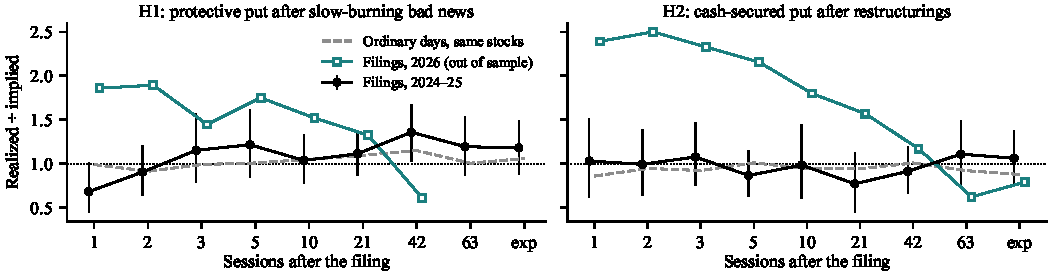
\includegraphics[width=\linewidth]{decay.pdf}
\vspace{-3ex}
\caption{Realized move divided by the move the chain priced on the session before the filing, with 95 percent intervals for 2024--25 filings; 1 means priced correctly.}
\label{fig:decay}
\end{figure}

\textbf{A fresh year.} On 2022, run once, H1 beat ordinary days by 4.30 percent at 21 sessions [$+0.54$, $+7.93$] on 12 events and met both conditions at that horizon, but not at 42 sessions or expiry, so it does not pass. Splitting the position shows why, and it is not H1's mechanism: after the bad news the stocks rose 6.1 percent in 21 sessions, with only a quarter falling, against 0.6 percent on ordinary days, while the put alone lost 1.8 percent. In a falling market the headline was oversold and the put dear, and the protective put earned through the stock it owns. A filter to the most liquid names, set before the run, left too few events (3 and 1).

\section{Sensitivity, costs and capacity}
At 21 sessions the H2 edge is positive in all 9 cells of expiry bucket by out-of-money distance (3, 5, 10 percent), $+0.08$ to $+1.24$ percent, and H1 in 7 of 9, $-0.67$ to $+0.68$. By tag (exploratory, at most 15 events each), only restructuring plans with the sold put clear zero: $+2.57$ percent at expiry [$+0.95$, $+4.51$]. A 5 percent premium charge each way costs 28 to 29 basis points of the stock price, and quoted half-spreads where Massive has quotes are 26 to 29; net of the charge the edge is about $+11$ basis points for both families. Per trade at 21 sessions, annualized, the in-sample Sharpe ratio is 1.20 for H1 and 1.41 for H2 after the charge, against 1.20 and 1.13 for the same strategies on ordinary days before it; H2 out of sample is $-1.36$. The median put traded 34 (H1) and 49 (H2) contracts on the entry day, so at 10 percent participation a trader fills 3 to 5 contracts per event, about \$0.1 million of stock, on about one event per family a month.

\section{What would break it, and what we predicted}
Samples are small, the company list is today's, spot is inferred from the chain and marks are daily last trades. Before running any unseen window we committed a forecast: it called no pass and the H2 count out of sample, and missed the H1 count (3 against about 11), the interval widths and all three signs it could score. \textbf{For the judges' sealed window it predicts} about 4 H1 and 3 H2 events in three months, so \emph{insufficient} for both, and a null for both in six months or more; a pass would contradict it.


\textbf{How to trade it.} We would not trade either rule. A holder who wants protection after these filings can buy it at the next close without overpaying by more than the bounds above. Next tests, each committed before its data: restructuring plans with the sold put, H2 entry after the first-week move, and post-filing rebounds in falling markets.



\end{document}
